\chapter{Avaliação}
\label{cap:avaliacao}

Neste capítulo será apresentado o processo de avaliação utilizado para verificar se os objetivos previstos foram alcançados. Espera-se que com a criação do modelo de usuário baseados em múltiplos domínios, haja uma melhoria na qualidade das recomendações. Para isso, os experimentos aqui relatados utilizam o Facebook\footnote{http://www.facebook.com} como fonte de dados do usuário e a DBpedia\footnote{http://www.dbpedia.org} como fonte de dados para os domínios de filmes e livros. A avaliação consiste em comparar as combinações de diferentes tipos de metadados, utilizando o algoritmo BPR-Mapping, apresentado no Capítulo \ref{cap:userModel}.

Este capítulo apresenta os detalhes da metodologia utilizada para desenvolver e avaliar este trabalho, bem como o conjunto de dados utilizados durante os experimentos. Em seguida são apresentadas as métricas utilizadas na avaliação e os resultados obtidos. Por fim, é feita uma discussão e apresentados pontos de melhoria.


\section{Metodologia}


Os testes realizados para a avaliação têm por objetivo mostrar que ao utilizar novos atributos, os quais podem ser provenientes de diferentes domínios, o sistema de recomendação conseguirá aumentar a precisão das recomendações.

Para avaliação do modelo serão realizadas comparações da combinação de diferentes tipos de metadados. As combinações utilizadas são: anos de nascimento e países, livros e países, cidades e países, sexo e países, anos de nascimento e gêneros, livros e gêneros, cidades e gêneros e, por fim, sexo e gêneros. Essas combinações são descritas em um arquivo de texto que contém relações binárias entre as entidades. Os arquivos com as relações contêm exatamente duas colunas, sendo que cada coluna tem o ID que identifica a entidade no banco de dados. Na Figura \ref{fig:movie-genre-file}, por exemplo, é representada a relação entre filme e gênero, em que a primeira linha corresponde ao filme 1 que é do gênero 3, a segunda linha ao filme 1 que é do gênero 5 e assim por diante.

\begin{figure}
	\centering
	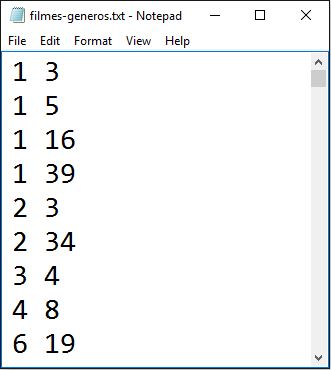
\includegraphics[scale=0.45]{imagens/movie-genre.png}
	\caption{Exemplo de arquivo da relação entre filme e gênero. Figura elaborada pelo autor (2015).}
	\label{fig:movie-genre-file}
\end{figure}

Os arquivos com as relações serão utilizados como entrada para o algoritmo BPR-Mapping descrito em \ref{sec:brp-mapping} através da biblioteca MyMediaLite \citep{gantner2011}. Para medir a melhoria das recomendações, foram utilizadas as métricas \ac{MAP} e \ac{AUC}.



\section{Conjunto de Dados}

Todos os testes foram executados com dados de usuários do Facebook \footnote{Facebook, http://www.facebook.com}. De cada usuário, foram coletados os filmes e livros que este marcou no Facebook como assistido ou lido, respectivamente, e armazenados com identificador, título e URLs do Facebook. Como o Facebook fornece poucos dados sobre os filmes e livros, foram extraídas informações adicionais da DBpedia, para enriquecer o conjunto de informações dos filmes e livros, com o objetivo de aumentar a precisão das recomendações.

Para coletar essas informações foi feita uma busca utilizando o nome de cada filme e livro do usuário na DBpedia, para então extrair as informações. Foi necessário modificar alguns dos nomes dos itens que vieram do Facebook, porque os nomes dos filmes estão em português e os dados disponibilizados na DBpedia estão em inglês. Para cada filme, são consultados o diretor, país, data de lançamento, sinopse, gêneros. Para cada livro são consultados autor, país, data de lançamento, sinopse, gêneros, número de páginas. O banco de dados final foi composto de 37 usuários relacionados a 9 cidades, 1189 filmes e 637 livros com relações entre 30 países e 39 gêneros, como pode ser visto na Tabela \ref{tab:conjunto-dados}


\begin{table}[]
	\centering
	\caption{Conjunto de Dados.}
	\label{tab:conjunto-dados}
	\begin{tabular}{|c|c|}
		\hline
		\multicolumn{2}{|c|}{\textbf{Conjunto de Dados}} \\ \hline
		usuários                  & 37                   \\ \hline
		cidades                   & 9                    \\ \hline
		filmes                    & 1189                 \\ \hline
		livros                    & 637                  \\ \hline
		países                    & 30                   \\ \hline
		gêneros                   & 39                   \\ \hline
	\end{tabular}
\end{table}


Para os teste foi utilizado o processo de \textit{cross-validation}, onde é criado conjuntos de treino e de teste, o modelo é treinado utilizando o conjunto de treino e testado com os exemplos do conjunto de teste. Em seguida, diferentes conjuntos de treino e teste são selecionados para iniciar o processo de treino e teste novamente, sendo repetido $k$ vezes \citep{ricci2011recommender}. Finalmente, a performance média é reportada. Existem várias técnicas de \textit{cross-validation}, aqui foi utilizada a técnica \textit{n-Fold}, o conjunto de dados é dividido em $n$ grupos. Um dos grupos é utilizado para testar o modelo e os restantes $n-1$ grupos são utilizados para treino. O processo de \textit{cross-validation} é então repetido $n$ vezes com cada uma das $n$ subamostragens utilizadas exatamente uma vez como dado de validação \citep{ricci2011recommender}.

O algoritmo utilizado foi o BPR-Mapping \ref{sec:brp-mapping}, o qual foi executado utilizando diferentes conjuntos de entradas, totalizando oito execuções. A primeira execução foi realizada sem utilizar atributos de filmes, livros ou do usuário, e será utilizada como base para avaliação de performance das outras sete execuções. Deste modo, são comparadas as notas de \ac{MAP} e \ac{AUC} obtidas ao utilizar os atributos dos filmes, livros e usuários com a nota gerada na primeira execução. Os resultados obtidos estão listados na Tabela \ref{tab:resultados}.





\section{Métricas de Avaliação}

Em um cenário onde é fornecida uma lista de recomendações a um usuário em que ele pode avaliar os itens como relevantes ou não-relevantes, métricas como Precisão \footnote{Em inglês, Precision.} e Cobertura \footnote{Em inglês, Recall.}, utilizadas na recuperação de informação, são úteis para avaliar a qualidade de um método de recomendação \citep{parra2013}.

Por exemplo, recomendações baseadas em tag dependem fortemente dessas métricas, já que os usuários não costumam indicar sua preferência dando notas aos itens \citep{Bogers:2009}.

Precisão é a fração dos itens recomendados que são relevantes \citep{Manning:2008:IIR:1394399}, sendo definida como

\begin{equation}
precisao = \frac{itens~relevantes~recomendados}{itens~na~lista}~~,
\end{equation}

Cobertura é definida como a fração de recomendações relevantes que são apresentadas para o usuário \citep{Manning:2008:IIR:1394399}

\begin{equation}
cobertura = \frac{itens~relevantes~recomendados}{itens~relevantes}~~,
\end{equation}

Entretanto, como descrito por \cite{Herlocker:2004:ECF:963770.963772}, \textit{cobertura} é inútil em seu puro sentido para avaliar sistemas de recomendação, uma vez que exige conhecer todos os itens que são relevantes para um usuário central. A Figura \ref{fig:precisaocobertura} ilustra estes conceitos.

\begin{figure}
	\centering
	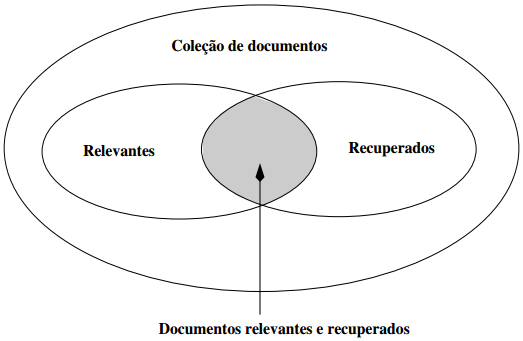
\includegraphics[scale=0.8]{imagens/precisao_cobertura.png}
	\caption{Precisão e Cobertura  \citep{DBLP:journals/rita/Barth13}.}
	\label{fig:precisaocobertura}
\end{figure}

\subsection{Precisão em n (Prec@n)}

O número de itens recomendados em uma lista pode ser muito alto, dependendo do método de recomendação e do tamanho do conjunto de dados, e um usuário pode não ser capaz de verificar e avaliar todos eles. Por esta razão, as métricas de avaliação irão considerar apenas os top itens, que são chamados Top-N recomendações \citep{Deshpande:2004:ITN:963770.963776}, e são normalmente apresentados como precisão em n (P@n). P@n é utilizado para avaliar o sistema no contexto de um único usuário. A \textit{P@n} mede a relevância dos $n$ primeiros itens de uma lista:

\begin{equation}
P@n = \frac{r}{n}~~,
\end{equation}

onde, $n$ é o número de itens retornados e $r$ é o número de itens considerados relevantes e retornados até a posição $n$ da lista.

\subsection{\textit{Mean Average Precision} (MAP)}
A fim de obter uma métrica única que contribui para a precisão do método de recomendação ao longo de todo o conjunto de usuários, utiliza-se o \textit{Mean Average Precision (MAP)} \citep{parra2013}. \ac{MAP} é obtida calculando a média sobre a precisão média da lista de recomendações de cada usuário, como:

\begin{equation}
MAP = \sum_{n=1}^{N}\frac{AveP(n)}{N}~~,
\end{equation}

onde, $AveP(n)$ é a precisão média para o usuário $n$, isto é, a média dos valores de precisão obtidos para o conjunto de top-N recomendações depois que cada recomendação relevante é recuperada \citep{Manning:2008:IIR:1394399}.

\subsection{\textit{Area Under the ROC curve} (AUC)}

Métricas de classificação são apropriadas para tarefas como "Encontrar Bons Itens", especialmente quando apenas avaliações implícitas estão disponíveis, isto é, nós sabemos quais itens um usuário gostou, mas não o quanto eles gostaram. Para avaliar este tipo de sistemas, uma métrica popular é \ac{AUC}, onde ROC significa \textit{Receiver Operating Charachteristics} \citep{hanley1982mau}. A métrica \ac{AUC} tenta medir como um sistema de recomendação pode distinguir com sucesso os itens relevantes (aqueles apreciados pelo usuário) dos itens irrelevantes (todos os outros) \citep{DBLP:journals/corr/abs-1202-1112}.

A maneira mais fácil de calcular \ac{AUC} é comparando a probabilidade que os itens relevantes serão recomendados com a dos itens irrelevantes \citep{DBLP:journals/corr/abs-1202-1112}. Para $n$ comparações independentes (cada comparação refere-se a escolher um item relevante e um irrelevante), se existem $n'$ vezes em que o item relevante tem uma nota alta em relação ao irrelevante e $n''$ vezes em que as notas são iguais, então de acordo com \cite{zhou2009predicting}:

\begin{equation}
AUC = \frac{n'~+~0.5n''}{n}~~,
\end{equation}

Claramente, se todos os itens relevantes tiverem nota maior do que os irrelevantes, AUC = 1 o que significa uma lista de recomendação perfeita. Para uma lista de recomendação aleatória, AUC = 0,5. Portanto o grau em que AUC excede 0,5 indica a habilidade de um algoritmo de recomendação em identificar itens relevantes.







\section{Resultados}

Para avaliar os resultados foram utilizadas as seguintes métricas de avaliação:

\begin{enumerate}[label=(\alph*)]
	\item Precisão, que calcula	o percentual de itens recomendados que são relevantes;
	\item \ac{MAP}, que calcula a precisão considerando a respectiva posição na lista ordenada de itens recomendados e;
	\item \ac{AUC}, que especifica a probabilidade de que, ao tirar um exemplo negativo e outro positivo aleatoriamente, a função de decisão atribua um valor mais alto para o positivo do que o exemplo negativo.
\end{enumerate}

\subsection{Prec@5}

O prec@5 considera a precisão dos cinco primeiros itens na lista, pontuando mais os acertos no início. Analisando os resultados obtidos, o nível de melhoria chegou a 91,31\%, o que é um valor bem expressivo.

\begin{table}[]
	\centering
	\caption{Resultados para AUC, prec@5 e prec@10.}
	\label{tab:resultados}
	\begin{tabular}{|c|c|c|c|c|c|}
		\hline
		\textbf{Atributos do Filme} 	& \textbf{Atributos do Usuário} & \textbf{AUC} 		& \textbf{prec@5} 	& \textbf{prec@10} 	& \textbf{MAP} 		\\ \hline
		sem atributos                   & sem atributos            		& 0,76189      		& 0,01888         	& 0,02120  			& 0,06719          	\\ \hline
		países                			& sem atributos            		& 0,77813      		& 0,02388         	& 0,02370  			& 0,07261          	\\ \hline
		gêneros               			& sem atributos            		& 0,77977      		& 0,02388         	& 0,02390  			& 0,07899         	\\ \hline
		países                			& ano de nascimento          	& 0,78743      		& 0,03244         	& 0,02616  			& 0,08193        	\\ \hline
		países                			& livros              			& 0,79902      		& 0,03544         	& \textbf{0,02916} 	& 0,08838         	\\ \hline
		países                			& cidades             			& 0,78898      		& 0,03494         	& 0,02491  			& 0,08683        	\\ \hline
		países                			& sexo            				& 0,77762      		& 0,03244         	& 0,02366  			& 0,07984         	\\ \hline
		gêneros                   		& ano de nascimento          	& 0,78450      		& 0,01888         	& 0,02120  			& 0,05977         	\\ \hline
		gêneros                   		& livros              			& \textbf{0,80516}	& 0,02388         	& 0,02370   		& \textbf{0,09154}  \\ \hline
		gêneros                   		& cidades             			& 0,78079      		& \textbf{0,03612} 	& 0,02845  			& 0,08231      		\\ \hline
		gêneros                   		& sexo            				& 0,78602      		& 0,02388         	& 0,02370  			& 0,07414         	\\ \hline
	\end{tabular}
\end{table}

O maior valor alcançado com o prec@5 foi obtido ao utilizar os atributos gênero do filme e cidade do usuário, alcançando um valor de 0,03612, como pode ser visto na Tabela \ref{tab:resultados}. Isto se deve provavelmente ao fato de que muitos dos usuários registrados na aplicação pertenciam a cidades em comum ou eram amigos na rede social Facebook, o que nos leva a acreditar que podem ter interesses em comum por filmes.


Porém, houve um caso em que não houve melhoria, o valor obtido ficou igual ao valor do teste sem atributos. Foi o caso em que se utilizou os atributos gênero do filme e data de nascimento do usuário, obtendo uma nota de 0,01888. Isto pode ser devido ao fato de que o ano de nascimento entre os usuários é esparso, ou seja, em alguns casos não foi informado.



\subsection{Prec@10}

No prec@10 a performance não foi tão grande comparada ao prec@5, já que este considera os dez primeiros itens da lista. O nível de melhoria alcançado com o prec@10 foi de 37,55\% e, mesmo sendo mais baixo que o prec@5, ainda assim é um bom resultado.

O maior valor alcançado pelo prec@10 foi obtido ao utilizar os atributos país do filme e livros do usuário, obtendo um valor de 0,2916. Podemos deduzir, neste caso, o interesse dos usuários por filmes e livros de uma mesma nacionalidade, sendo os itens de maior interesse de nacionalidade estadunidense.


\begin{figure}
	\centering
	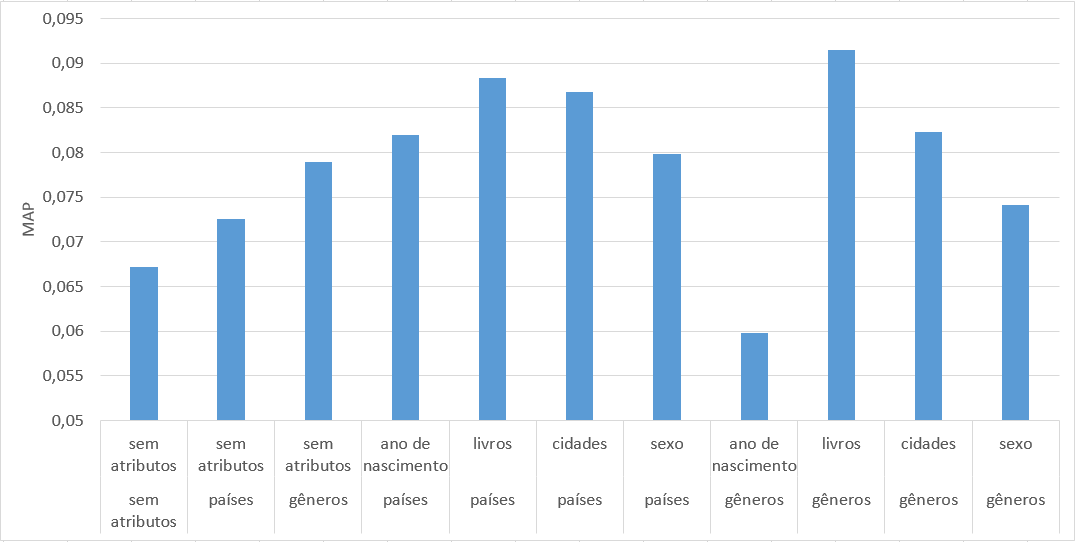
\includegraphics[scale=0.55]{imagens/grafico_map.png}
	\caption{Resultados da métrica MAP utilizando o algoritmo BPR-Mapping. Figura elaborada pelo autor (2015).}
	\label{fig:grafico_map}
\end{figure}

Como no prec@5, o prec@10 também não mostrou melhoria ao utilizar os atributos gênero do filme e data de nascimento do usuário, obtendo uma nota de 0,01888, mesma nota do teste sem atributos.


\subsection{MAP}

A métrica \ac{MAP} foi utilizada para medir a precisão do algoritmo. Analisando os resultados obtidos pelo \ac{MAP} na Tabela \ref{tab:resultados}, o nível de melhoria ficou entre 8,07\% e 36,24\%. Estas melhorias são significativas, já que aumentar o \ac{MAP} é um problema difícil, e cada aumento é difícil de se alcançar.

Os valores obtidos ao utilizar os atributos dos filmes, livros e usuário são geralmente muito melhores. O maior valor alcançado com o \ac{MAP} foi obtido ao utilizar os atributos gênero do filme e livros do usuário, alcançando um valor de 0,09154, visto na Figura \ref{fig:grafico_map}. Isso se deve provavelmente ao fato de que as relações entre filmes e livros podem ser facilmente conectadas, como por exemplo, um usuário que gostou de um livro de terror tende a gostar de filmes de terror.

Contudo, houve um caso em que o valor foi mais baixo que o do teste sem utilizar atributos, que foi ao utilizar os atributos gênero do filme e data de nascimento do usuário, que obteve um valor de 0,05977, valor 11\% menor. Isto deve-se, provavelmente, ao fato de que o ano de nascimento pode influenciar no interesse em determinados gêneros de filmes, por exemplo, pessoas mais velhas tendem a gostar mais de filmes clássicos do que um jovem.

\subsection{AUC}


\begin{figure}
	\centering
	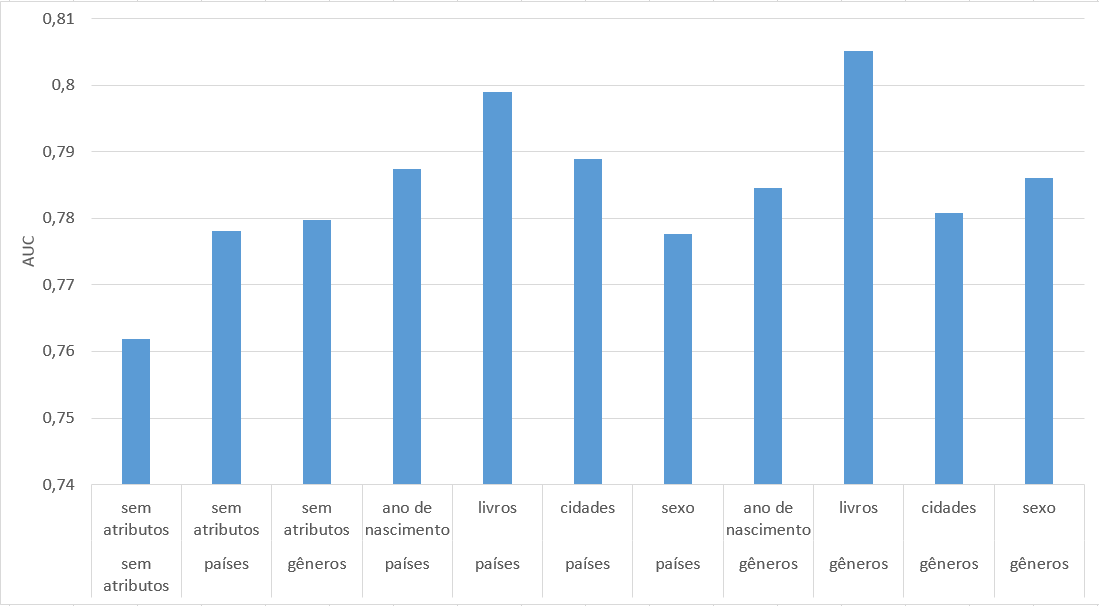
\includegraphics[scale=0.5]{imagens/grafico_auc.png}
	\caption{Resultados da métrica AUC utilizando o algoritmo BPR-Mapping. Figura elaborada pelo autor (2015).}
	\label{fig:grafico_auc}
\end{figure}

Para a métrica \ac{AUC} o melhor valor possível a ser obtido seria 1, e qualquer ranking não aleatório que faça sentido tem valores AUC > 0,5. Nos testes realizados, todos os valores obtidos pela métrica AUC estiveram acima de 0,5.

Analisando os valores na Tabela \ref{tab:resultados}, obtidos com a métrica \ac{AUC}, mais uma vez temos o maior valor alcançado ao utilizar os atributos gênero do filme e livros do usuário, atingindo um valor de 0,80516. Portanto o algoritmo foi capaz de identificar itens relevantes para recomendar ao usuário.




\section{Discussão}

Neste trabalho foi mostrado a modelagem de perfis de usuários em múltiplos domínios, e de forma automatizada, com o objetivo de transferir conhecimento sobre o usuário em um domínio para um outro domínio relacionado. Este conhecimento adicional pode ajudar a aliviar o problema da partida-a-frio, principalmente em casos de usuários novos, em que não há conhecimento sobre ele o suficiente para começar a gerar recomendações.

Após analisar os resultados obtidos com as métricas utilizadas, podemos concluir que compartilhar informações entre domínios aumenta a performance da recomendação consideravelmente. Combinar atributos dos filmes com os dos livros sempre produziu melhores resultados. Todos os testes realizados apresentaram melhorias significativas, como podem ser visto nas Figuras \ref{fig:grafico_map} e \ref{fig:grafico_auc}, ao utilizar os atributos de livros do usuário para realizar recomendações de filmes. Assim, podemos perceber o quanto a utilização de dados sobre outros domínios pode ajudar na precisão da recomendação, principalmente no que diz respeito ao problema da partida-a-frio (cold-start problem), já que o modelo de usuário é criado de forma automática com dados do usuário já disponíveis em redes sociais.

Uma rede social de filmes, como o Filmow\footnote{Filmow, http://www.filmow.com.br}, por exemplo, pode fazer uso da abordagem proposta neste trabalho para melhorar as recomendações de filmes que faz aos usuários de sua rede. Ao utilizar os dados sobre livros que seus usuários leram, no Facebook, ela pode fazer uso dessas informações adicionais para aumentar a precisão de suas recomendações, principalmente para novos usuários, em que começam sem ter filmes no perfil da rede.








\section{Pontos de Melhoria}

Os principais problemas na criação automática do modelo de usuário foram na etapa de coleta de outros dados sobre os itens a partir da DBpedia, após obter os filmes e livros do usuário do Facebook. Como o Facebook fornece apenas o nome do filme ou livro, a busca na DBpedia precisou ser realizada através do nome, o que trouxe problemas relacionados a erros de grafia ou ruídos, como em casos em que o ano do filme aparecia concatenado ao título. Muitos casos foram resolvidos, mas ainda restam muitos pontos para melhorias neste quesito.

Outro problema deve-se às informações dos filmes e livros estarem muitas vezes incompletas ou com pouca informação útil. Isso pode ser melhorado com a obtenção de dados sobre os itens em sites especializados, como IMDB\footnote{IMDB, http://www.imdb.com}, por exemplo. Outra possibilidade é a utilização de outras fontes de conhecimento sobre o usuário, como outras redes sociais que possam fornecer mais conhecimento sobre o usuário, como Twitter\footnote{Twitter, http://www.twitter.com}, Google Plus\footnote{Google+, https://plus.google.com/}, e outras.

O modelo do usuário ainda tem possibilidade de ser alimentado com muito mais informações que podem ser obtidas criando novas relações entre os domínios. Então existe muito espaço para explorar e gerar novos dados seguindo a abordagem apresentada neste trabalho.


\section{Sumário}

Este capítulo apresentou os principais resultados obtidos durante o desenvolvimento dos experimentos para avaliar a implementação de modelos de usuários baseados em múltiplos domínios, utilizando extração automática de informações dos usuários. Inicialmente foram apresentadas as metodologias de avaliação utilizadas no estudo, dataset, e métricas utilizadas. O estudo apresentado neste capítulo mostrou que a proposta de cruzar informações entre domínios foi efetivas em obter melhores recomendações para o usuário.